\documentclass{article}
\usepackage{nips_2016}
\usepackage[utf8]{inputenc} % allow utf-8 input
\usepackage[T1]{fontenc}    % use 8-bit T1 fonts
\usepackage{hyperref}       % hyperlinks
\usepackage{url}            % simple URL typesetting
\usepackage{booktabs}       % professional-quality tables
\usepackage{amsfonts}       % blackboard math symbols
\usepackage{nicefrac}       % compact symbols for 1/2, etc.
\usepackage{microtype}      % microtypography
\usepackage{graphicx}       % inserting images

\title{Self-driving cars in Duckietown environment\\[10pt]Önvezető autózás Duckietown környezetben}

\author{
  Endrész Balázs \\
  BME \\
  Budapest, Hungary\\
  \texttt{endresz.balazs@edu.bme.hu} \\
  \And
  Monori János Bence \\
  BME \\
  Budapest, Hungary \\  
  \texttt{monoribence@edu.bme.hu} \\
  \AND
  Wenesz Dominik \\
  BME \\
  Budapest, Hungary \\
  \texttt{dominik.wenesz@edu.bme.hu} \\
  %% \And
  %% Coauthor \\
  %% Affiliation \\
  %% Address \\
  %% \texttt{email} \\
  %% \And
  %% Coauthor \\
  %% Affiliation \\
  %% Address \\
  %% \texttt{email} \\
}

\begin{document}
\maketitle

\begin{abstract}
  Our task was to implement a reinforcement learning-based neural
  network for lane following in the Duckietown simulational environment.
  \textit{going straight, turning left and turning right}. Thus a \textit{Q-learning algorithm}
  was implemented. During every step a screenshot is taken which is followed by a segmentation
  process: the outer white line is filtered to a Blue channel while the yellow line
  in the middle to the Red channel. After this preprocessing method, a reward function is calculated
  for the three different actions and the one with the highest possible value is chosen.
  Our solution was by far not the most efficient approach to the problem, however several
  promising results are seen. \par
  A feladatunk az volt, hogy egy megerősítéses tanulás (RL) alapú neurális hálózatot
  hozzunk létre egy útvonalkövetéses problémára a Duckietown környezetben. Ehhez egy
  Q-hálót építettünk fel. Minden lépésben egy képernyőképet mentünk ki a szimulátorból,
  a képet szegmentáljuk: a külső folytonos vonalat a kék csatornára, míg a középső szaggatott
  vonalat a piros csatornára. A feldolgozást követően egy függvénnyel kiértékeljük az aktuális
  pillanatban legjobb tevékenységet. A mi megoldásunk messzemenőkig nem a legjobb megközelítés volt,
  ellenben rengeteg ígéretes eredmény született.
\end{abstract}

\section{Introduction}

\thispagestyle{empty}
In this semester our task was to create a self-driving AI and test it in  Duckietown
simulational environment. Reinforcement learning is widely used to problems in robotics,
and control engineering, involving self-driving cars, decision processes, and control systems. 
\par
The Duckietown Project was initiated in 2016 as an MIT graduate project.\cite{gym_duckietown} It contains
vehicles called Duckiebots which circulate around the town. In this project we can participate
in a bunch of challenges such as lane following, passing through intersections or controling
multiple Duckiebots at once. In this paper we will describe our methods on solving the
problems mentioned above and talk about the results.

%\subsection{On the Duckietown Fundation}
%The Duckietown Project was initiated in 2016 as an MIT graduate project, based on
%several different challenges such as lane following, object detecting, or passing
%intersections. This lead to the AI Driving Olympics where anyone could participate
%with their model, competing in the tasks mentioned before. A simulational environment
%is available in the official GitHub repository of the Duckietown Project, this
%functions as the base of model assembling and testing, hyperparameter optimization, 
%and predicting. Several solutions and dissertations are available online using 
%different approaches to the problem, but few to none mention Q-learning as a valid 
%method.  
\newpage
\section{The solution}
\subsection{Motivation}
Mentioned before: Q-learning was rarely implemented for this specific problem, 
so we chose to experiment using this method. Our motivation came from an AI 
beating Google Chrome's built-in dinosaur game.  The algorithm converged rapidly 
with appropriate image pre-processing, hence it seemed good to implement in the 
Duckietown environment.
\subsection{First try - pathfinding}
The gym contains a pathfinder file which can be completed with an arbitrary pathfinding algorithm
to circulate town. \cite{gym_duckietown}
Our first idea was to find the shortest path between two points on a given map and after
so a lane following agent could go through that. Hence an A* algorithm\cite{4082128} was implemented
to obtain a valid route, but this solution basically does not involve any neural networks, thus
it is scratched.
\subsection{Image preprocessing}
In the simulation in every step a screenshot is taken, preprocessed and after that it goes
into the convolutional neural network. First of all, we cut and resized the
pictures to 80x60 pixels, so the unnecessary data won't affect the agent's behaviour.
\begin{figure}[h]
  \centering
  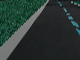
\includegraphics[scale=1.9]{fig2.png}
  \caption{The raw resized image.}
\end{figure}
\\
Our first approach to process these images was to
filter out the lines on the road, giving us a black and white picture as seen below.
To make the learning more efficient we have implemented a better segmentation algorithm.
In this case the outer white lines are filtered to the blue channel while the inner dashed
line is filtered to the red channel. This is managed in a HSV color model since OpenCV
supported this way better: lower and upper thresholds are given for the white and yellow
colors.\cite{CHOW197261,HARALICK1985100} If a pixel is within the pre-specified range then it is filtered to either the
blue or red channel. A mask is created such way which is merged with the raw picture,
and after that is normalized. The results can be seen below:
\begin{figure}[h]
  \centering
  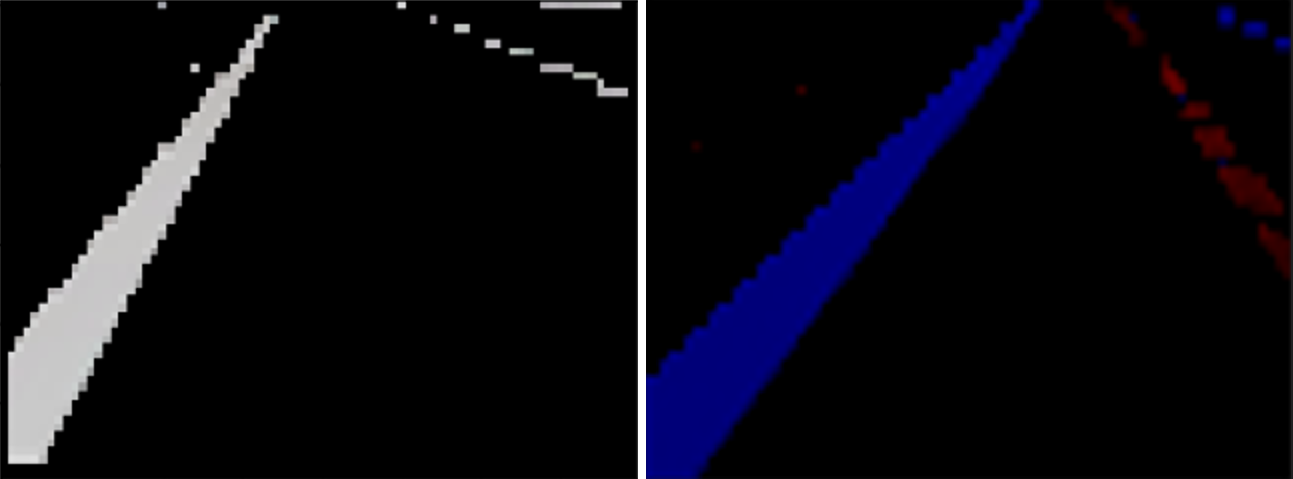
\includegraphics[scale=0.3]{fig1.png}
  \caption{The results from segmentation.}
\end{figure}
\subsection{The Convolutional Neural Network}
Since our task is based on visual elements, we have created a 2D Convolutional Network.\cite{lecun1995convolutional}
The network is based of the cited papers.\cite{Kalapos2020,kalapos2021vision,watkins1992q}
\begin{table}[h]
  
  \label{sample-table}
  \centering
  \begin{tabular}{lll}
    \toprule\toprule
    \multicolumn{2}{c}{Layer} \\
    \cmidrule{1-2}
    Name     & Shape    & Param  \\
    \midrule
    Conv2D & (58,78,32)  &  896    \\
    MaxPooling2D & (29,39,32)  &  0   \\
    Conv2D & (27,37,32)  &  9248    \\
    MaxPooling2D & (13,18,32)  &  0    \\
    Conv2D & (11,16,64)  &  18496    \\
    MaxPooling2D & (5,8,64)  &  0    \\
    Flatten & (2560)  &  0   \\
    Dense & (128)  &  327808    \\
    Dense & (3)  &  387    \\
    \bottomrule
  \end{tabular}\\[5pt]
  \caption{The CNN model}
\end{table}
\subsection{Q-learning}
In every step a screenshot is taken and based on the (1) equation, a value is calculated
for every possible action - \textit{going straight, turning left, turning right}:\cite{watkins1992q}
\begin{equation}
  Q'=Q+\alpha(r+\gamma\cdot \max Q_{est}-Q)
\end{equation}
where $Q'$ is the new value, $Q$ is the old value, $\alpha$ is the learning rate (which was chosen as 0.05)
$r$ is the reward, $\gamma$ is the discount factor (which is 0.95 in our case)\cite{even2003learning}, 
$Q_{est}$ is the estimated value to a given action. Using this function the best action
is chosen based on the reward function.\cite{kalapos2021vision,Kalapos2020}
\section{Results}
Our results didn't happen to be the best solution, however it seems like it is mostly just
a matter of time to achieve better results. The following graph shows the loss function:
\begin{figure}[h]
  \centering
  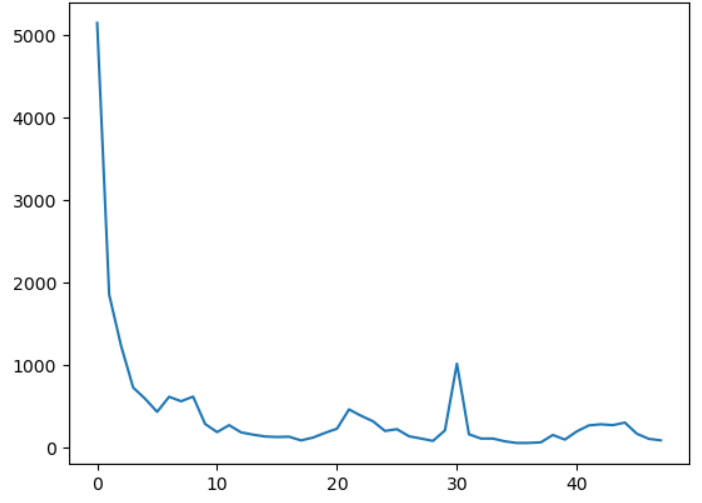
\includegraphics[scale=0.4]{LossFunction.png}
  \caption{The loss function.}
\end{figure}\\
We can clearly see that the method did converge, however it is by far not enough for a stable solution.
Several things can be done to get a better agent, such as using checkpointer, using a scheduler
which reduces the learning rate $\alpha$ over time. Also it should be emphasized that
our method was experimentary, and other reinforcement learning algorithms might
do better on this task.
\section{Conclusion}
In this paper we describer our methods to solve an interesting lane following problem
in the Duckietown simulational environment. We found that Q learning might not be the
best solution to this problem nonetheless it seems promising. We showed that this can
be a viable approach even if a bunch of things could be implemented to achieve better
results.

\section*{Acknowledgement}
We would like to thank all the professors and PhD students for all the assistance and
guide given to us. Altough our solution is not perfect, it was a very interesting task
to work on, and we feel grateful for the learning experience.

\nocite{*}
\bibliographystyle{plain}
\bibliography{refs.bib}

\end{document}